\documentclass[t, pdftex]{beamer}  
%Use Cockrell School Theme.  Optional department name.  Must %ecape, i.e. use 
%backslash, to preserve spaces.  The default is ``Cockrell School of Engineering''                 
\usetheme[dept=Aerospace\ Engineering\ and\ Engineering\ Mechanics]{cockrell}                          
\usepackage{animate}
\usepackage{amsmath}
\expandafter\patchcmd\csname beamerx@\string\beamer@framefootnotetext\endcsname
  {\color@begingroup}
  {\color@begingroup\toggletrue{blx@footnote}}
  {\togglefalse{blx@tempa}}
  {}
% Add preamble packages here


%Enable cancelto in math
\usepackage{cancel}
\renewcommand{\CancelColor}{\color{utorange}}
\let\svthefootnote\thefootnote
%Add bibliography file location for citition
\bibliography{example.bib}


\title{Impact of ice-shelf channels on ice sheet/shelf instability}
\subtitle{}
\author{ Julius LOOS}
\vspace{0,9cm}
\institute{\textbf{Master Thesis}\vspace{0,4cm} \\Supervision:\\Reinhard Drews, Clemens Schannwell, Todd Ehlers}
\date{\today}

\setbeamertemplate{footline}[frame number]
\setlength\abovecaptionskip{0.05ex}
\setlength\belowcaptionskip{-2.5ex} % a re-changer si besoin de gagner de la place encore
\setbeamercolor{background canvas}{bg=yellow!10!white}


\begin{document}

%Creates title frame from title, subtitle, author, institute, and date above
\begin{frame}[noframenumbering, plain]
\titlepage
\end{frame}

%\frame{\frametitle{Outline}\vfill\tableofcontents\vfill}

%\section{Introduction}

%\begin{frame}
	%\frametitle{Introduction}
    %\begin{columns}
    %\begin{column}{.45\linewidth}
    %\underline{Important notions : }
    %\vspace{.5cm}
	%\begin{itemize}
	%	\item Ice shelf mass balance and stability % Define it 
	%	\item Channel evolution and and their contribution to ice shelf disintegration  % IceShelf/Sheet stability
     %   \item Sea level rise
%	\end{itemize}
 %   \bigskip
  %  \begin{description}
%				\item[WAIS : ]{West Antarctic ice-sheet}
%				% Altitude minimum : -2500m
%				% Formed during the late Cainozoic
%			\end{description}
 %   \end{column}
  %  \begin{column}{.65\linewidth}
   % \vspace{-0.5cm}
    %\begin{figure}
%    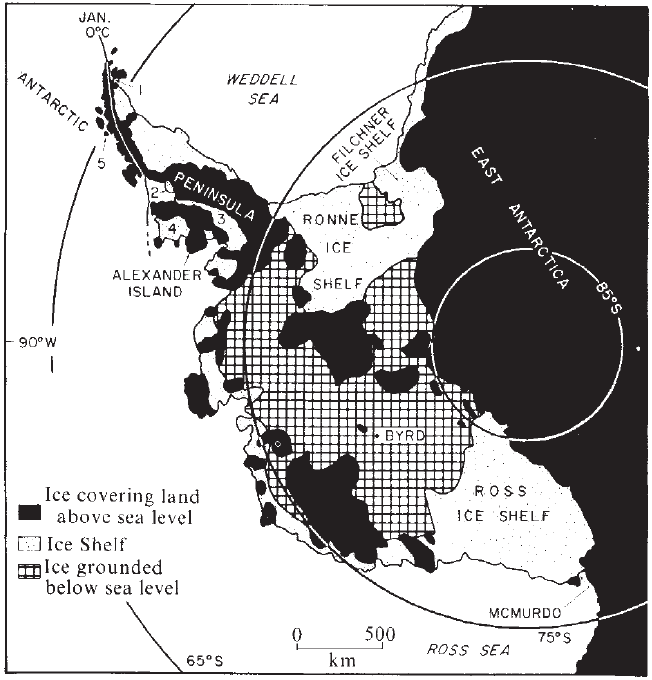
\includegraphics[scale = 0.33]{figure2_mercer.png}
%    \caption{Marine ice-sheet in West Antarctica}
%    \end{figure}
%    \end{column}
%    \end{columns}
%    \footfullcite{mercer1978}
    % Had to consist of cold ice from the start (mercer) + issue because the destabilization is really quick so no time for the coastal cities to adjust different with East Antarctica.
	% There are more and more parameters so reassessments of what models predicted.
%\end{frame}
 
\section{Introduction}
\begin{frame}
	\frametitle{Introduction}
	\begin{itemize}
		\item   Transition from grounded ice sheet to floating ice shelf $\rightarrow$ defined by grounding line
		\item   Ice shelf mass balance and stability 
	\end{itemize}
    \vspace{0.2cm}
      \begin{figure}
   % 	\only<1>{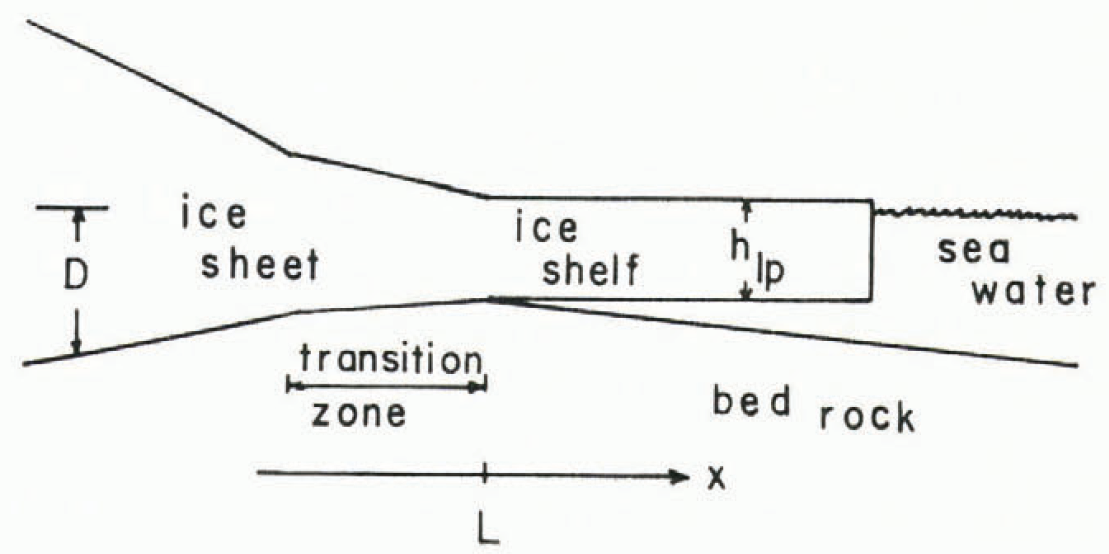
\includegraphics[width = .7\textwidth]{figure3_weertman.png}}
        \only<1>{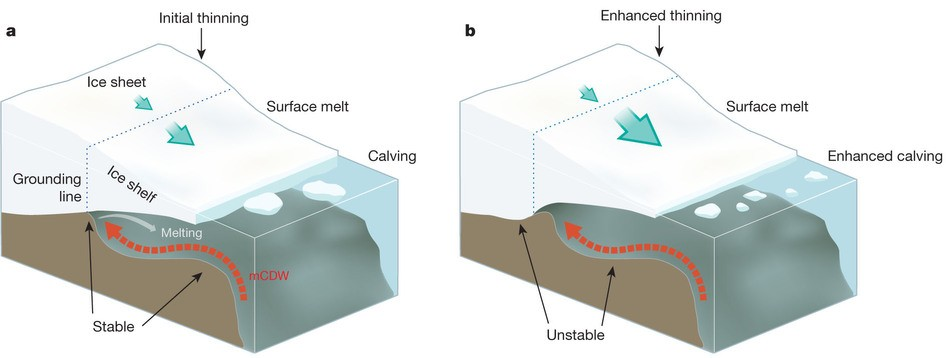
\includegraphics[width = 1\textwidth]{ice.jpg}}
    	%\caption{Circum polar deep waters enhance basal melting and thinning of the ice shelf.}
    \end{figure}
    \vspace{-.3cm}
    \footfullcite{hannah}         
\end{frame}
   
\subsection{Ice shelf instability}
\begin{frame}
	\frametitle{Ice shelf instability}
    \textcolor{utorange}{\textbf{$\rightarrow$ Flux is an increasing function of the ice thickness}}
    	\begin{equation}
	\nonumber
	\tcbhighmath[boxrule=2pt,arc=1pt,colback=yellow!2!white,colframe=black,
		drop fuzzy shadow=red]{q= f[h(L)]}
	\end{equation}
    \vspace{-.3cm}
        \begin{figure}
    	\only<1>{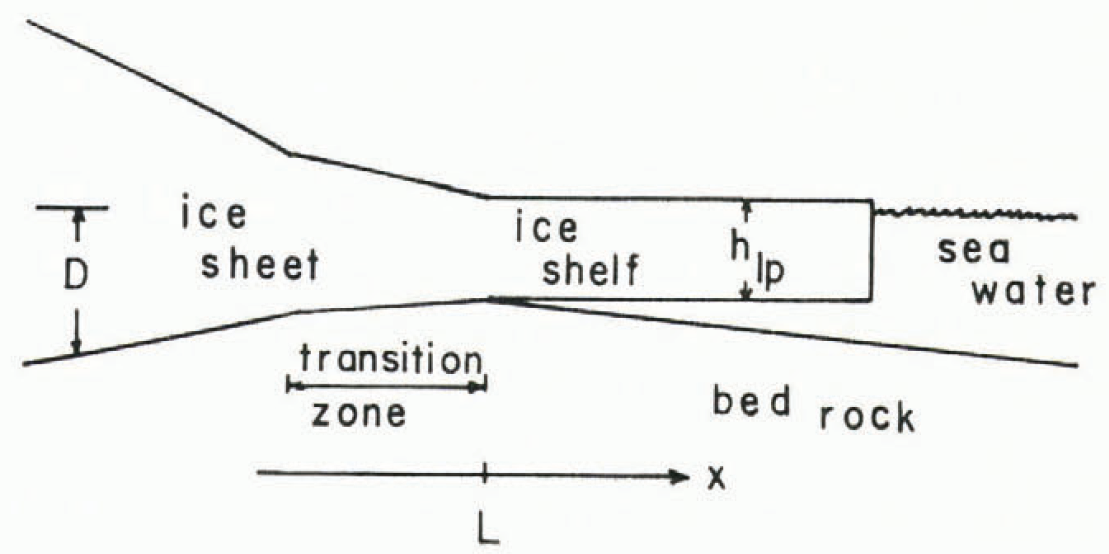
\includegraphics[width = .7\textwidth]{figure3_weertman.png}}
        %\only<2>{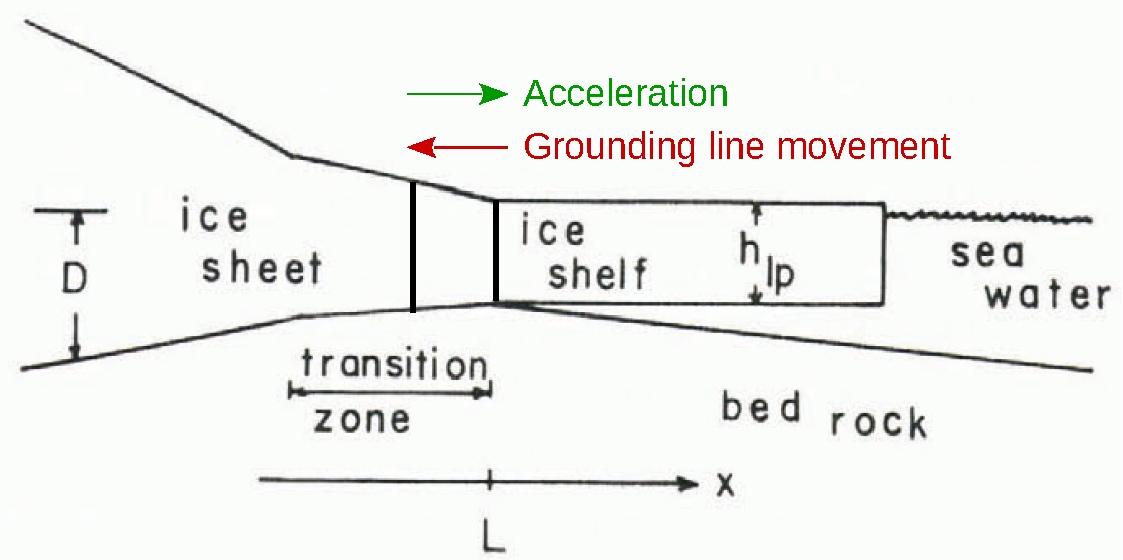
\includegraphics[width = .7\textwidth]{retrograde_weertman.pdf}}
    	%\caption{Weertman (1974)}
    \end{figure}
    \footfullcite{weertman1974}
    
%Discharge is controlled by ice dynamics – the faster the ice flows across the grounding line, the larger the discharge will be, as well as the flux is an increasing function of thickness of the ice.  Positive feedback loop 
\end{frame}
   
   
   
   
\subsection{Ice shelf channels}
\begin{frame}
	\frametitle{Ice shelf channels}
	\begin{itemize}
		\item Longitudinal ice shelf channels, which often start near the grounding line
		\begin{itemize}
		\item Thin ice sections where channels are located
		\end{itemize} % Define it 
		\item Buttressing of the continental ice flux through ice shelves
	\end{itemize}
    \vspace{0.2cm}
      \begin{figure}
   % 	\only<1>{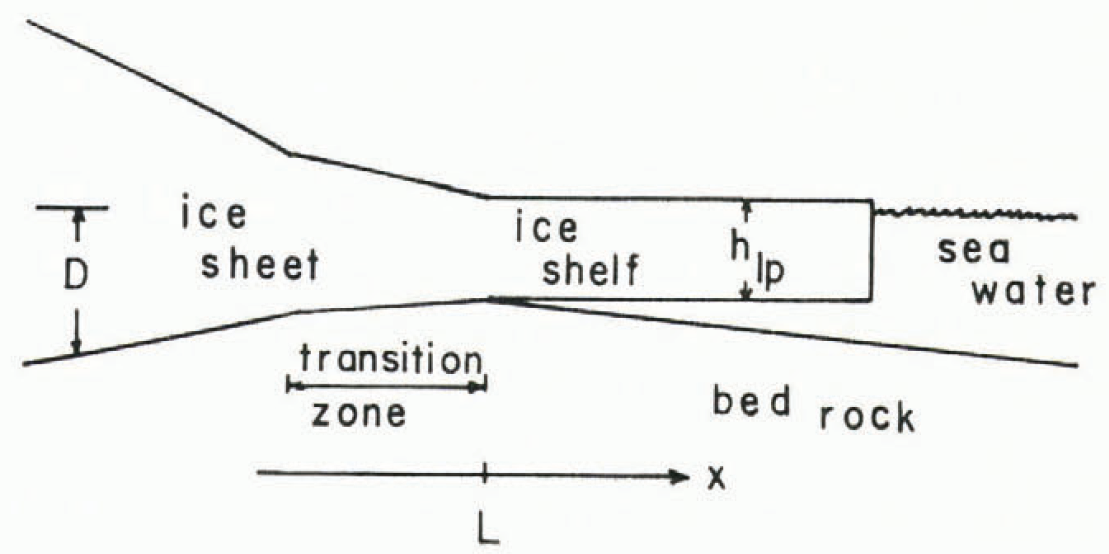
\includegraphics[width = .7\textwidth]{figure3_weertman.png}}
        \only<1>{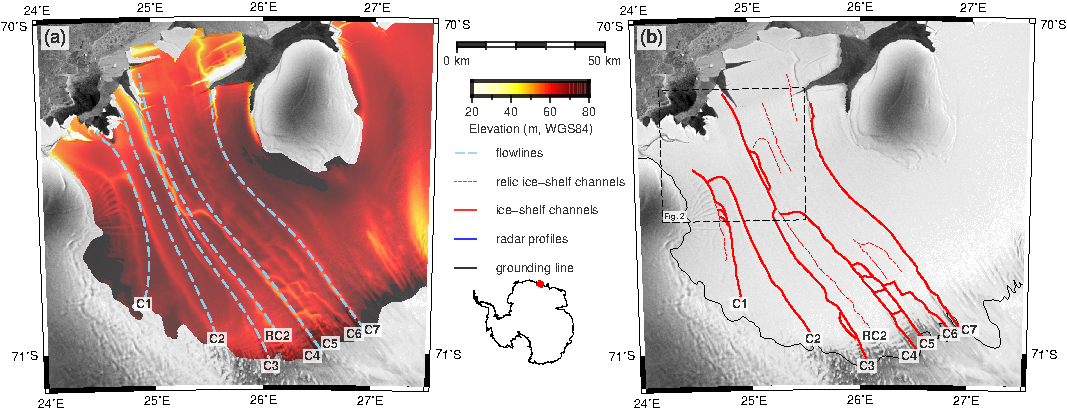
\includegraphics[width = 1\textwidth]{channels.pdf}}
    %	\caption{}
    \end{figure}
    \vspace{-.3cm} 
    \let\thefootnote\relax\footnote{Image source: Reinhard Drews}      
\end{frame}


\begin{frame}
	\frametitle{Ice shelf channels}
	\begin{itemize}
		\item Longitudinal ice shelf channels, which often start near the grounding line
		\begin{itemize}
		\item Thinner ice sections where channels are located
		\end{itemize} % Define it 
		\item Basal melting indicates channel creation
	\end{itemize}
    \vspace{0.2cm}
      \begin{figure}
   % 	\only<1>{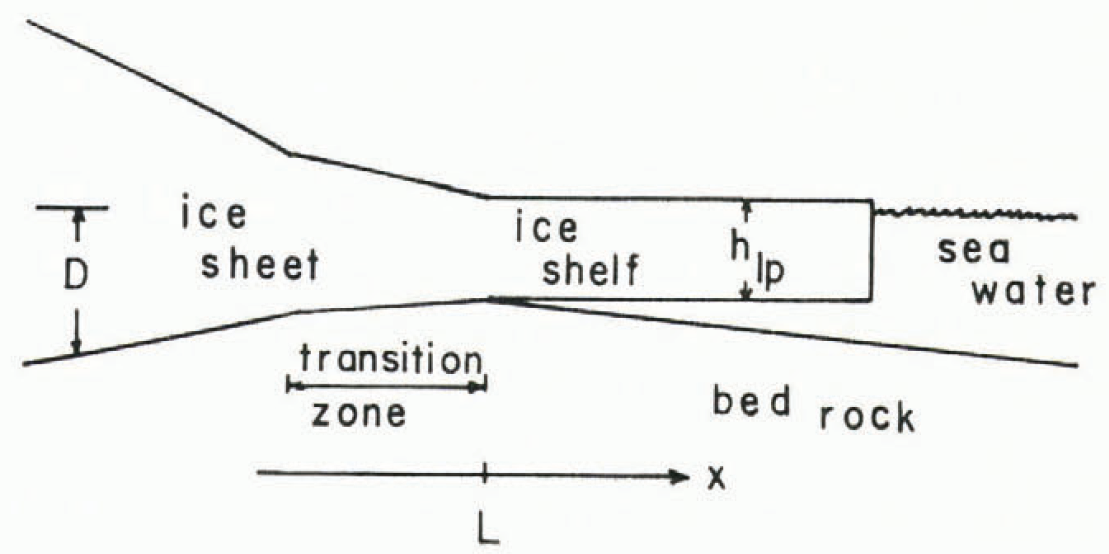
\includegraphics[width = .7\textwidth]{figure3_weertman.png}}
        \only<1>{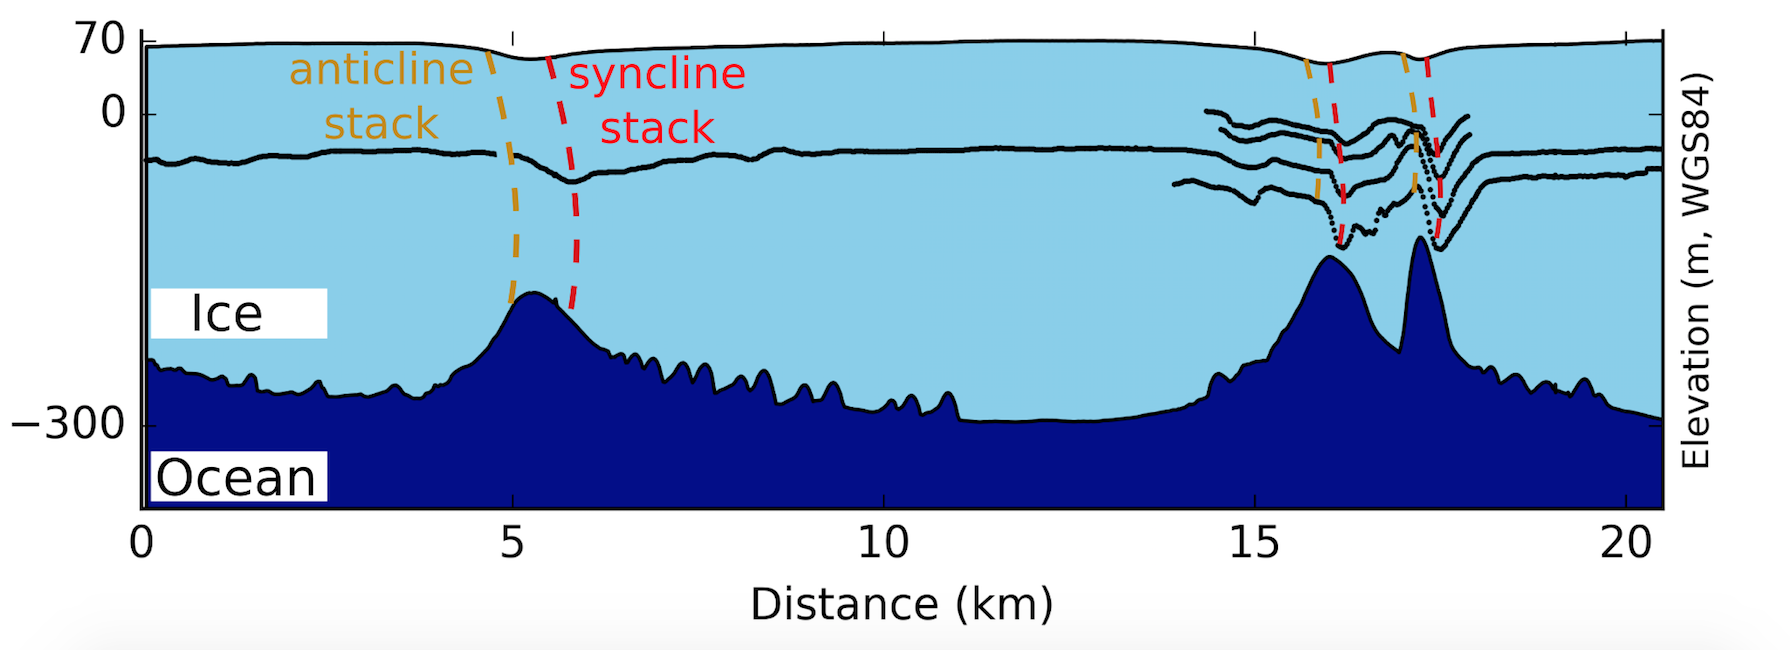
\includegraphics[width = 1\textwidth]{Figs_SimAn/channel_2.png}}
    	%\caption{}
    \end{figure}
    \vspace{-.3cm}
    \let\thefootnote\relax\footnote{Image source: Reinhard Drews}        
\end{frame}
 

\section{Methods}
\begin{frame}
	\frametitle{Methods/ Scientifc Outline}
	\vspace{0,4cm}
    \textcolor{utorange}{\textbf{$\rightarrow$ Numerical simulation using Elmer/Ice}} \\
\vspace{0,2cm}   
 \begin{itemize}
 \setlength\itemsep{1em}
 \item Full stokes, finite element, ice sheet / ice flow model 
 \item Constructing a three dimensional synthetic model
 			\begin{itemize}
 			\item Adjustment of parameter and model geometry
 			\item Implementing ice shelf channels
 			\end{itemize}
 			 \end{itemize}
		 
\textcolor{utorange}{\textbf{$\rightarrow$ Scientific outline}} 
\vspace{0,2cm}  
\begin{itemize} 				
 \item Ice channel propagation and preservation 
 \item In general: Link to ice shelf disintegration and ice shelf instability
\end{itemize}
\end{frame}


\begin{frame}[noframenumbering, plain]
	\frametitle{Thank you for your attention}
    \vfill
    \centerline{
\includegraphics[scale = 1]{question.jpg}} 
    \vfill
\end{frame}

\begin{frame}[noframenumbering, plain]
	\frametitle{References}
	\vspace{0,4cm}
	\item \cite{weertman1974}
	\item \cite{drews2015}
	\item \cite{hannah}
\end{frame}

\end{document}
